\documentclass[tikz, border=2mm, rgb]{standalone}
\usepackage[utf8]{inputenc}
\usepackage[T1]{fontenc}
\usepackage{lmodern}
\usepackage{xcolor}
\usetikzlibrary{shapes.geometric, shapes.symbols, positioning, calc, fit, backgrounds, arrows.meta}

\begin{document}
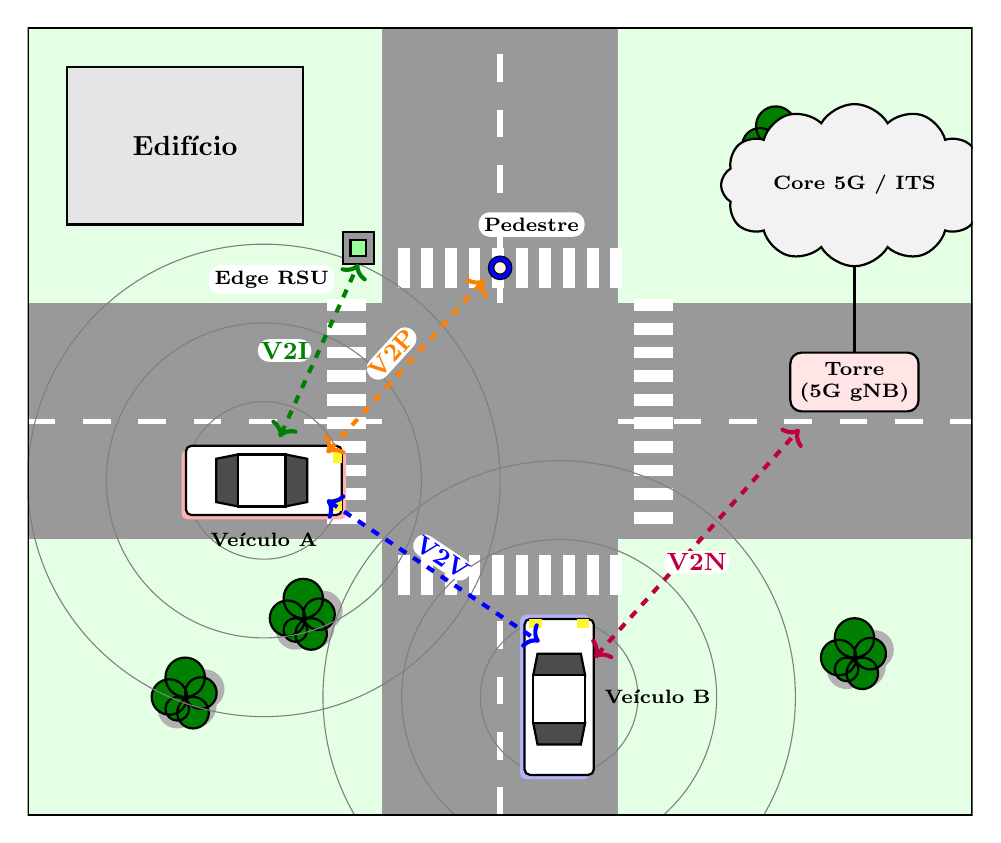
\begin{tikzpicture}[
    font=\sffamily,
    car top up/.pic={
        \begin{scope}[scale=0.55]
            \filldraw[fill=blue!30, draw=none, rounded corners=2pt] (-0.9, -1.9) rectangle (0.7, 1.9);
            \filldraw[fill=white, draw=black, rounded corners=2pt, thick] (-0.8, -1.8) rectangle (0.8, 1.8);
            \filldraw[fill=black!70, draw=black, thick] (-0.6, 0.5) -- (-0.5, 1.0) -- (0.5, 1.0) -- (0.6, 0.5) -- cycle;
            \filldraw[fill=black!70, draw=black, thick] (-0.6, -0.6) -- (-0.5, -1.1) -- (0.5, -1.1) -- (0.6, -0.6) -- cycle;
            \filldraw[fill=white, draw=black, thick] (-0.6, -0.6) rectangle (0.6, 0.5);
            \filldraw[fill=yellow!80, draw=none] (-0.7, 1.6) rectangle (-0.4, 1.8);
            \filldraw[fill=yellow!80, draw=none] (0.4, 1.6) rectangle (0.7, 1.8);
        \end{scope}
    },
    car top right/.pic={
        \begin{scope}[scale=0.55]
            \filldraw[fill=red!30, draw=none, rounded corners=2pt] (-1.9, -0.9) rectangle (1.9, 0.7);
            \filldraw[fill=white, draw=black, rounded corners=2pt, thick] (-1.8, -0.8) rectangle (1.8, 0.8);
            \filldraw[fill=black!70, draw=black, thick] (0.5, -0.6) -- (1.0, -0.5) -- (1.0, 0.5) -- (0.5, 0.6) -- cycle;
            \filldraw[fill=black!70, draw=black, thick] (-0.6, -0.6) -- (-1.1, -0.5) -- (-1.1, 0.5) -- (-0.6, 0.6) -- cycle;
            \filldraw[fill=white, draw=black, thick] (-0.6, -0.6) rectangle (0.5, 0.6);
            \filldraw[fill=yellow!80, draw=none] (1.6, -0.7) rectangle (1.8, -0.4);
            \filldraw[fill=yellow!80, draw=none] (1.6, 0.4) rectangle (1.8, 0.7);
        \end{scope}
    },
    tree/.pic={
        \begin{scope}[scale=0.5]
            \fill[black!30] (0.2,-0.2) circle (0.6) (-0.2,-0.3) circle (0.5) (0.5,0.2) circle (0.5);
            \filldraw[fill=green!50!black, draw=black, thick]
                (0,0.5) circle (0.5)
                (0.4, 0.1) circle (0.4)
                (-0.4, 0) circle (0.45)
                (0.2, -0.4) circle (0.4)
                (-0.2, -0.3) circle (0.3);
        \end{scope}
    }
]

    % Clip to bounding box
    \clip (0,0) rectangle (12,10);

    % Background grass / terrain
    \fill[green!10] (0,0) rectangle (12,10);

    % Crossroads (Streets)
    % Vertical street (x=4.5 to 7.5)
    \fill[black!40] (4.5, 0) rectangle (7.5, 10);
    % Horizontal street (y=3.5 to 6.5)
    \fill[black!40] (0, 3.5) rectangle (12, 6.5);
    
    % Street markings (White dashed lines)
    \draw[line width=2pt, white, dashed, dash pattern=on 10pt off 10pt] (6, 0) -- (6, 3.5);
    \draw[line width=2pt, white, dashed, dash pattern=on 10pt off 10pt] (6, 6.5) -- (6, 10);
    \draw[line width=2pt, white, dashed, dash pattern=on 10pt off 10pt] (0, 5) -- (4.5, 5);
    \draw[line width=2pt, white, dashed, dash pattern=on 10pt off 10pt] (7.5, 5) -- (12, 5);
    
    % Crosswalks
    \foreach \y in {3.7, 4.0, 4.3, 4.6, 4.9, 5.2, 5.5, 5.8, 6.1, 6.4} {
        \fill[white] (3.8, \y) rectangle (4.3, \y+0.15); % Left
        \fill[white] (7.7, \y) rectangle (8.2, \y+0.15); % Right
    }
    \foreach \x in {4.7, 5.0, 5.3, 5.6, 5.9, 6.2, 6.5, 6.8, 7.1, 7.4} {
        \fill[white] (\x, 2.8) rectangle (\x+0.15, 3.3); % Bottom
        \fill[white] (\x, 6.7) rectangle (\x+0.15, 7.2); % Top
    }

    % Objects (Trees, Buildings)
    \filldraw[fill=gray!20, draw=black, thick] (0.5, 7.5) rectangle (3.5, 9.5);
    \node[font=\bfseries, align=center] at (2, 8.5) {Edifício};

    % Trees
    \pic at (2, 1.5) {tree};
    \pic at (3.5, 2.5) {tree};
    \pic at (9.5, 8.5) {tree};
    \pic at (10.5, 2) {tree};

    % Car 1 (Going Right on horizontal street)
    % Center: x=3.0, y=4.25
    \foreach \r in {1, 2, 3} { \draw[black!50, thin] (3, 4.25) circle (\r); }
    \pic at (3, 4.25) {car top right};
    \node[font=\scriptsize\bfseries] at (3, 3.5) {Veículo A};

    % Car 2 (Going Up on vertical street)
    % Center: x=6.75, y=1.5
    \foreach \r in {1, 2, 3} { \draw[black!50, thin] (6.75, 1.5) circle (\r); }
    \pic at (6.75, 1.5) {car top up};
    \node[font=\scriptsize\bfseries] at (8.0, 1.5) {Veículo B};

    % V2I RSU (Traffic light / Edge node at intersection corner)
    \filldraw[fill=gray!80, draw=black, thick] (4.0, 7.0) rectangle (4.4, 7.4);
    \filldraw[fill=green!40, draw=black, thick] (4.1, 7.1) rectangle (4.3, 7.3);
    \node[fill=white, inner sep=2pt, font=\scriptsize\bfseries, rounded corners] at (3.1, 6.8) {Edge RSU};

    % V2N Tower & Cloud (Top Right)
    \node[draw=black, fill=red!10, thick, rounded corners, align=center, font=\scriptsize\bfseries] (Tower) at (10.5, 5.5) {Torre\\(5G gNB)};
    \node[cloud, cloud puffs=12, cloud puff arc=120, aspect=2, draw=black, fill=gray!10, thick, font=\scriptsize\bfseries] (Cloud) at (10.5, 8.0) {Core 5G / ITS};
    \draw[thick] (Tower) -- (Cloud);

    % V2P Pedestrian (Crossing top crosswalk)
    \filldraw[fill=blue] (6.0, 6.95) circle (0.15); 
    \filldraw[fill=white!80!pink] (6.0, 6.95) circle (0.08); 
    \node[fill=white, inner sep=2pt, font=\scriptsize\bfseries, rounded corners] at (6.4, 7.5) {Pedestre};

    % Communication Links
    % V2V (Car 1 <-> Car 2)
    \draw[<->, dashed, line width=1.5pt, blue] (3.8, 4.0) -- (6.5, 2.2) node[midway, sloped, above=1pt, fill=white, inner sep=1pt, rounded corners, font=\bfseries\small] {V2V};
    
    % V2I (Car 1 <-> RSU)
    \draw[<->, dashed, line width=1.5pt, green!50!black] (3.2, 4.8) -- (4.2, 7.0) node[midway, left=2pt, fill=white, inner sep=1pt, rounded corners, font=\bfseries\small] {V2I};
    
    % V2N (Car 2 <-> Tower)
    \draw[<->, dashed, line width=1.5pt, purple] (7.2, 2.0) -- (9.8, 4.9) node[midway, below=2pt, fill=white, inner sep=1pt, rounded corners, font=\bfseries\small] {V2N};
    
    % V2P (Car 1 <-> Pedestrian)
    \draw[<->, dashed, line width=1.5pt, orange] (3.8, 4.6) -- (5.8, 6.8) node[midway, sloped, above=2pt, fill=white, inner sep=1pt, rounded corners, font=\bfseries\small] {V2P};

    % Border 
    \draw[thick] (0,0) rectangle (12,10);

\end{tikzpicture}
\end{document}
